\subsection{Struttura del progetto}
	\subsubsection{Server}
	
	\begin{figure}[H]
		\centering
		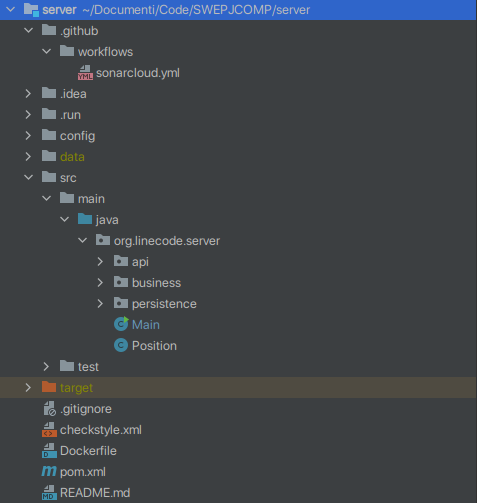
\includegraphics[width=10cm]{img/struttura_server.png}
		\caption{Struttura del server}
	\end{figure}

	\begin{itemize}
		\item{.github}: contiene le configurazioni per la CI in ambiente github;
		\item{.idea}: contiene le configurazioni generali per l'IDE IntellijIDEA;
		\item{.run}: contiene le configurazioni per l'esecuzione del codice all'interno	dell'IDE IntellijIDEA;
		\item{config}: contiene gli script di inizializzazione del database;
		\item{src}: contiene i sorgenti dell'applicativo, suddivisi di default dal framework in 2 sotto	directory:
		\begin{enumerate}
			\item{main}: contiene una folder per ciascun layer:
				\begin{itemize}
					\item{api}: strato per la connessione e la comunicazione con l'interfaccia e l'unità;
					\item{business}: strato della logica dell'elaborazione dati;
					\item{persistence}: strato di comunicazione tra il server e il database;
				\end{itemize}
			\item{test}: contiene i test di unità;
		\end{enumerate}
		\item{target}: contiene i file compilati;
	\end{itemize}

	Troviamo inoltre nella root della directory i seguenti file:
	\begin{itemize}
		\item{Dockerfile}: per la generazione della DockerImage da eseguire in ambiente Docker;
		\item{pom.xml}: il file di progetto di Maven;
		\item{checkstyle.xml}: file di configurazione di Checkstyle;
	\end{itemize}

\newpage

	\subsubsection{Interfaccia}
	
	\begin{figure}[H]
		\centering
		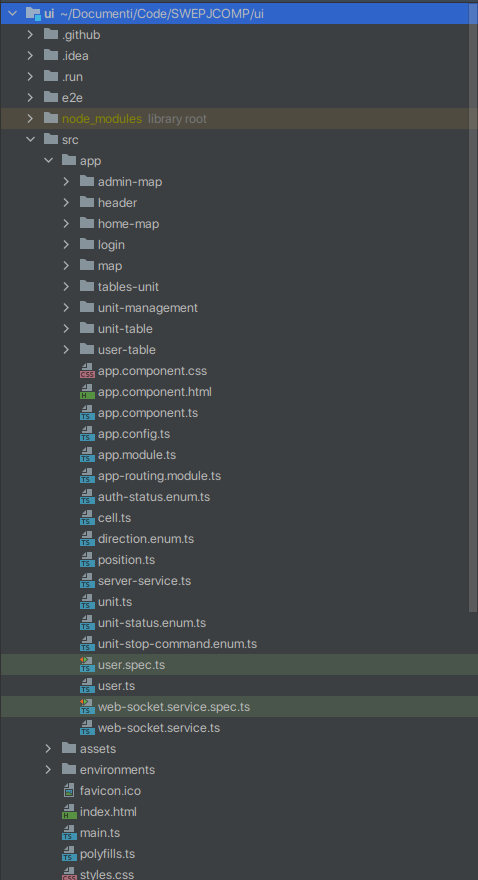
\includegraphics[width=10cm]{img/struttura_ui.png}
		\caption{Struttura della UI}
	\end{figure}

	\begin{itemize}
		\item{.github}: contiene le configurazioni per la CI in ambiente github;
		\item{.idea}: contiene le configurazioni generali per l'IDE IntellijIDEA;
		\item{.run}: contiene le configurazioni per l'esecuzione del codice all'interno	dell'IDE IntellijIDEA;
		\item{e2e}: contiene le configurazioni di base per i test end-to-end (e2e) del sito, utilizzati per tracciare i comportamenti dell'utente sul sito durante il testing;
		\item{node\_modules}: contiene i moduli di NodeJS installati tramite NPM e necessari all'esecuzione del codice. Per installarli eseguire il comando npm install dopo aver scaricato la repo;
		\item{src}: contiene i sorgenti dell'applicativo, suddivisi di default dal framework in 3 sotto	directory:
		\begin{enumerate}
			\item{app}: contiene una folder per ciascun componente sviluppato (es. componente unit-table ha una folder unit table) all'interno della quale si trovano 3 file, che contengono html css e logiche del component (file scritto in .ts). Oltre a questi	contiene singoli file .ts (typescript) che formano il model della ui applicativo;
			\item{assets}: contiene i file multimediali (se usati) impiegati nella realizzazione della UI;
			\item{environments}: contiene le specifiche di configurazione per gli ambienti di sviluppo e rilascio della UI.
		\end{enumerate}
	\end{itemize}

	Troviamo inoltre nella root della directory i seguenti file:
	\begin{itemize}
		\item{index.html}: pagina in html che funge da entrypoint per l'applicativo;
		\item{main.ts}: file Typescript che funge da entrypoint per l'avvio dell'applicativo (che segue le specifiche dell'ambiente di sviluppo);
		\item{styles.css}: file che contiene le specifiche di stile globali all'intero progetto.
	\end{itemize}

	All'interno della root della ui troviamo poi i seguenti file, in aggiunta a quelli della configurazione di default del progetto che avviene con Angular CLI:
	\begin{itemize}
		\item{Dockerfile}: per la generazione della DockerImage da eseguire in ambiente Docker;
		\item{package.json}: specifica i moduli e la configurazione dell'ambiente NodeJS per l'esecuzione dell'applicativo;
		\item{karma.conf.js}: file di configurazione per la suite di test;
		\item{sonar-project.properties}: file di configuazione per l'analisi statica attraverso il sito	SonarCloud.
	\end{itemize}

\newpage

	\subsubsection{Unità}
	
	\begin{figure}[H]
		\centering
		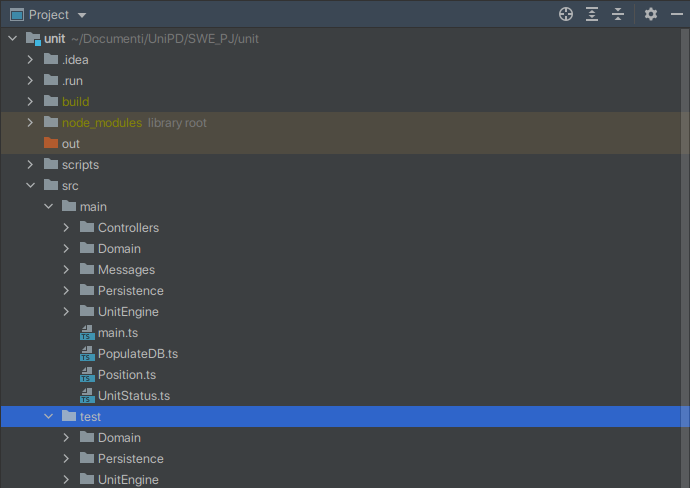
\includegraphics[width=10cm]{img/struttura_unita.png}
		\caption{Struttura dell'unità}
	\end{figure}

	\begin{itemize}
		\item{.idea}: contiene le configurazioni generali per l'IDE IntellijIDEA;
		\item{.run}: contiene le configurazioni per l'esecuzione del codice all'interno dell'IDE IntellijIDEA;
		\item{build}: contiene i file compilati da TS a JS dei sorgenti contenuti in src;
		\item{node\_modules}: contiene i moduli di NodeJS installati tramite NPM e	necessari all'esecuzione del codice. Per installarli eseguire il comando npm install dopo aver scaricato la repo;
		\item{scripts}: contiene script utili al popolamento del database per la persistenza dei dati;
		\item{src}: cartella dei sorgenti, divisa tra:
		\begin{itemize}
			\item{main}: codice di produzione dell'applicativo, suddiviso nelle cartelle Controllers (comunicazione), Domain e UnitEninge (logica interna), Messages (messaggi ricevuti e inviati al server), Persistence (persistenza dei dati);
			\item{test}: codice di test, suddiviso nelle cartelle Domain (test su logiche interne),	UnitEngine (sempre test su logiche interne) e Persistence (test sulla persistenza dei dati).
		\end{itemize}
	\end{itemize}
	
	Troviamo inoltre nella root della directory i seguenti file:
	\begin{itemize}
		\item{Dockerfile}: per la generazione della DockerImage da eseguire in ambiente Docker;
		\item{package.json}: specifica i moduli e la configurazione dell'ambiente NodeJS per l'esecuzione dell'applicativo.
	\end{itemize}

\newpage
	
\subsection{Aggiunta librerie}

\subsection{Aggiornamento librerie}

\subsection{Manutenzione dei test}
